\begin{figure}[H]
    \centering
    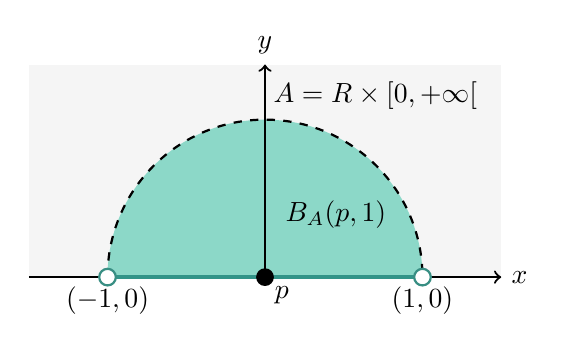
\begin{tikzpicture}[scale=2]
        % Semiplano A
        \fill[gray!8] (-1.5,0) rectangle (1.5,1.35);

        % Bola ambiente intersectada com A
        \fill[Emerald!45] (-1,0) arc (180:0:1) -- cycle;

        % Fronteira circular da bola ambiente
        \draw[dashed,thick] (-1,0) arc (180:0:1);

        % Eixos
        \draw[->,thick] (-1.5,0)--(1.5,0) node[right]{$x$};
        \draw[->,thick] (0,0)--(0,1.35) node[above]{$y$};

        % Diâmetro pertencente à bola do subespaço
        \draw[Emerald!75!black, ultra thick] (-1,0)--(1,0);

        % Extremidades abertas
        \draw[fill=white, draw=Emerald!70!black, thick] (-1,0) circle (1.5pt);
        \draw[fill=white, draw=Emerald!70!black, thick] (1,0) circle (1.5pt);

        % Centro
        \filldraw[black] (0,0) circle (1.5pt);
        \node[below right] at (0,0) {$p$};

        % Labels
        \node at (0.7,1.15) {$A=\mathbb R\times[0,+\infty[$};
        \node at (0.45,0.4) {$B_A(p,1)$};
        \node[below] at (-1,0) {$(-1,0)$};
        \node[below] at (1,0) {$(1,0)$};
    \end{tikzpicture}
    \caption{Bola aberta no subespaço $A=\mathbb R\times[0,+\infty[$.}
    \label{fig:bolaAbertaSubespaco}
\end{figure}
